\documentclass{article}

% Language setting
\usepackage[polish]{babel}

% Set page size and margins
% Replace `letterpaper' with `a4paper' for UK/EU standard size
\usepackage[letterpaper,top=2cm,bottom=2cm,left=3cm,right=3cm,marginparwidth=1.75cm]{geometry}

% Useful packages
\usepackage{amsmath}
\usepackage{graphicx}
\usepackage[T1]{fontenc}
\usepackage[colorlinks=true, allcolors=blue]{hyperref}
\usepackage{lipsum}
\usepackage{multicol}

\title{Metoda klasyfikacji cukierków na podstawie ich opakowania}
\author{Aleksander Golus, Bartosz Chadryś, Jakub Miśko, Igor Joński}

\begin{document}
\maketitle

\begin{abstract}
Praca przedstawia metodę klasyfikacji cukierków na podstawie ich opakowania. W pierwszej części opisany został temat projektu. Następnie, we wstępie opisane zostały wcześniejsze podejścia do problemu wraz z rozwiązaniami i celami. W trzeciej sekcji opisany został schemat układu pomiarowego, wraz z wykorzystanymi przedmiotami oraz szczegółowy opis zastosowania metody. Następnie opisane zostały wyniki pomiarów oraz ich analiza. Na podstawie wyników pomiarów w kolejnym rozdziale zostały rozpisane wnioski z przeprowadzonych pomiarów. Na samym końcu znajduje się bibliografia.
\end{abstract}

\section{Temat projektu}
Tematem projektu jest klasyfikacja cukierków na podstawie koloru ich opakowania. W tym celu został stworzony układ pomiarowy z taśmy produkcyjnej, kamery oraz zestawu konkretnych, prostokątnych, cukierków o kolorowych opakowaniach. Następnie została stworzona metoda rozróżniająca opakowania cukierków na podstawie ich koloru oraz zliczająca wystąpienia tych opakowań na podstawie ich koloru.

\section{Wstęp}
Detekcja obiektów przy użyciu OpenCV i Pythona jest bardzo powszechnie wykorzystywaną metodą. Nie ciężko jest znaleźć wiele przykładów na jej wykorzystanie w różnych dziedzinach. Przykładowo -

\section{Materiały i metody}
\subsection{Materiały pomiarowe}
Materiałami pomiarowymi są konkretne cukierki o kolorowych opakowaniach, to znaczy - cukierki marki Mamba oraz Turbo. Wykorzystywane cukierki dzielimy na 4 kolory, z czego różowy, czerwony oraz pomarańczowy to cukierki marki Mamba, natomiast zielony - marki Turbo. Rozmiar cukierka ma co prawda bezpośredni wpływ na to, czy jest on zakwalikifowany przez program czy nie, jednakże jego wymiary nie są jedyną rzeczą braną pod uwagę - o czym więcej w sekcji \ref{Metoda pomiarowa}.

\subsection{Układ pomiarowy}

Układ pomiarowy składa się z ciemnozielonej taśmy produkcyjnej napędzanej silnikiem elektrycznym o stałej prędkości, kamery o rozdzielczości 1080p oraz lampy LED naświetlającej taśmę z góry.
Taśma produkcyjna charakteryzuje się szerokością 10cm oraz stałą prędkością 3m/s. Oświetlona została lampą ledową o mocy 10W i temperaturze 3500K, co skutkuje klarownym oświetleniem bez zaburzenia kolorów cukierków.
Kamera została ustawiona 20cm nad taśmą, rejestrując przy tym całą szerokość taśmy.
Układ pomiarowy został przedstawiony na rysunku \ref{fig:uklad_pomiarowy}.

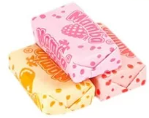
\includegraphics[width=5cm]{mamba.png}

\includegraphics[width=5cm]{gumaturbo.png}


\section{Wyniki i dyskusja}

\section{Wnioski}

\section{Literatura}

\begin{thebibliography}{9}
\bibitem{gfg}
\url{https://www.geeksforgeeks.org/detect-an-object-with-opencv-python/}

\bibitem{dry}
\url{https://dontrepeatyourself.org/post/color-based-object-detection-with-opencv-and-python/}

\bibitem{yt-motorcycle}
\url{https://www.youtube.com/watch?v=O3b8lVF93jU/}

\bibitem{yt-banana}
\url{https://www.youtube.com/watch?v=aFNDh5k3SjU&t=1004s/}

\end{thebibliography}

\section{Ściągawka}
Your introduction goes here! Simply start writing your document and use the Recompile button to view the updated PDF preview. Examples of commonly used commands and features are listed below, to help you get started.

Once you're familiar with the editor, you can find various project settings in the Overleaf menu, accessed via the button in the very top left of the editor. To view tutorials, user guides, and further documentation, please visit our \href{https://www.overleaf.com/learn}{help library}, or head to our plans page to \href{https://www.overleaf.com/user/subscription/plans}{choose your plan}.


\subsection{How to create Sections and Subsections}

Simply use the section and subsection commands, as in this example document! With Overleaf, all the formatting and numbering is handled automatically according to the template you've chosen. If you're using the Visual Editor, you can also create new section and subsections via the buttons in the editor toolbar.


\subsection{How to include Figures}

First you have to upload the image file from your computer using the upload link in the file-tree menu. Then use the includegraphics command to include it in your document. Use the figure environment and the caption command to add a number and a caption to your figure. See the code for Figure \ref{fig:frog} in this section for an example.

Note that your figure will automatically be placed in the most appropriate place for it, given the surrounding text and taking into account other figures or tables that may be close by. You can find out more about adding images to your documents in this help article on \href{https://www.overleaf.com/learn/how-to/Including_images_on_Overleaf}{including images on Overleaf}.


\subsection{How to add Tables}

Use the table and tabular environments for basic tables --- see Table~\ref{tab:widgets}, for example. For more information, please see this help article on \href{https://www.overleaf.com/learn/latex/tables}{tables}.

\begin{table}
\centering
\begin{tabular}{l|r}
Item & Quantity \\\hline
Widgets & 42 \\
Gadgets & 13
\end{tabular}
\caption{\label{tab:widgets}An example table.}
\end{table}


\subsection{How to add Comments and Track Changes}

Comments can be added to your project by highlighting some text and clicking ``Add comment'' in the top right of the editor pane. To view existing comments, click on the Review menu in the toolbar above. To reply to a comment, click on the Reply button in the lower right corner of the comment. You can close the Review pane by clicking its name on the toolbar when you're done reviewing for the time being.

Track changes are available on all our \href{https://www.overleaf.com/user/subscription/plans}{premium plans}, and can be toggled on or off using the option at the top of the Review pane. Track changes allow you to keep track of every change made to the document, along with the person making the change.


\subsection{How to add Lists}

You can make lists with automatic numbering \dots

\begin{enumerate}
\item Like this,
\item and like this.
\end{enumerate}
\dots or bullet points \dots
\begin{itemize}
\item Like this,
\item and like this.
\end{itemize}

\subsection{How to write Mathematics}

\LaTeX{} is great at typesetting mathematics. Let $X_1, X_2, \ldots, X_n$ be a sequence of independent and identically distributed random variables with $\text{E}[X_i] = \mu$ and $\text{Var}[X_i] = \sigma^2 < \infty$, and let
\[S_n = \frac{X_1 + X_2 + \cdots + X_n}{n}
  = \frac{1}{n}\sum_{i}^{n} X_i\]
denote their mean. Then as $n$ approaches infinity, the random variables $\sqrt{n}(S_n - \mu)$ converge in distribution to a normal $\mathcal{N}(0, \sigma^2)$.

\end{document}